\documentclass[reprint,amsmath,amssymb,aps,showpacs,superscriptaddress,prl]{revtex4-1}

\usepackage{graphicx}
\usepackage{bm}
\usepackage{epsfig}
\usepackage{amssymb}
\usepackage{amsfonts}
\usepackage{braket}
\usepackage{color}
\usepackage{epstopdf}
\epstopdfsetup{update}
\usepackage{hyperref}
\usepackage{float}
\restylefloat{table}
\usepackage{bibentry}
\usepackage{multirow}
\usepackage[caption=false]{subfig}
\newcommand{\ba}{\begin{eqnarray}}
\newcommand{\ea}{\end{eqnarray}}
\newcommand{\bd}{\begin{displaymath}}
\renewcommand{\v}[1]{{\bf #1}}
\newcommand{\nn}{\nonumber \\}

\graphicspath{{figures/}}% Put all figures in this directory.

\begin{document}
%
\title{Machine Learning Application to Two-Dimensional Dzyaloshinskii-Moriya Ferromagnets}

\author{Vinit Kumar Singh}
\email[Electronic address:$~~$]{vinitsingh911@gmail.com}
\affiliation{Department of Physics, Indian Institute of Technology, Kharagpur 721302, India}
\author{Jung Hoon Han}
\email[Electronic address:$~~$]{hanjemme@gmail.com}
\affiliation{Department of Physics, Sungkyunkwan University, Suwon 16419, Korea}
\date{\today}

\begin{abstract}
Principles of machine learning are applied to spin configurations generated by Monte Carlo method on Dzyaloshinskii-Moriya ferromagnetic models hosting the skyrmion phase in two dimensions. Successful feature predictions regarding the average spin chirality, magnetization, as well as magnetic field and temperature, were possible with the machine-learning architecture consisting of convolutional and dense neural network layers. Algorithms trained solely on the $xy$- or $z$-component of the local magnetization were as effective as the one trained on the full $xyz$ component of the input spin configuration in predicting various features. The predictive capacity of the algorithm extended beyond those configurations generated by the model used to make the training configurations, but also those generated by models plagued with disorder. A ``scaling procedure" for working with data generated at various length scales is developed, and proven to work in a manner analogous to the real-space renormalization process. 
\end{abstract}
%\pacs{75.78.-n, 75.10.Hk, 75.70.Kw, 75.78.Cd}
\maketitle

Enormous attention has been devoted to the application of machine learning (ML) ideas to various problems of condensed matter, particularly in regard to identifying many-body phases of classical and quantum models~\cite{melko16,wang16,melko17,melko17b,melko17c,tanaka17,scalettar17,wetzel17,wetzel17b,iso18,kim18,zhai17,scalettar17,beach18,zhai18,russian18}.
Following the natural progression in the level of sophistication, models studied with the ML method have evolved from Ising~\cite{melko16,wang16,melko17,melko17b,melko17c,tanaka17,scalettar17,wetzel17,wetzel17b,iso18,kim18} to planar (XY)~\cite{zhai17,scalettar17,wetzel17b,beach18,zhai18}, and most recently to Heisenberg~\cite{russian18} spins. At first, images - either quantum wave functions or classical configurations - are generated numerically. Then such images are fed to the deep learning architecture like the one shown in Fig. \ref{fig:1}, with key physical properties such as the order parameter and topological number as the information used to ``train" the algorithm. Once the training is complete, the algorithm is capable of predicting the same physical parameters for new images, called test sets, drawn from a similar pool of circumstances but which have never been used in the training. Problems to which such supervised learning has been applied so far have found fantastic success in the machine's predictive capacity. On the other hand, it seems to be the case that the success we witnessed does not extend beyond the confirmation of knowledge already known by other means.
%
\begin{figure}[ht]
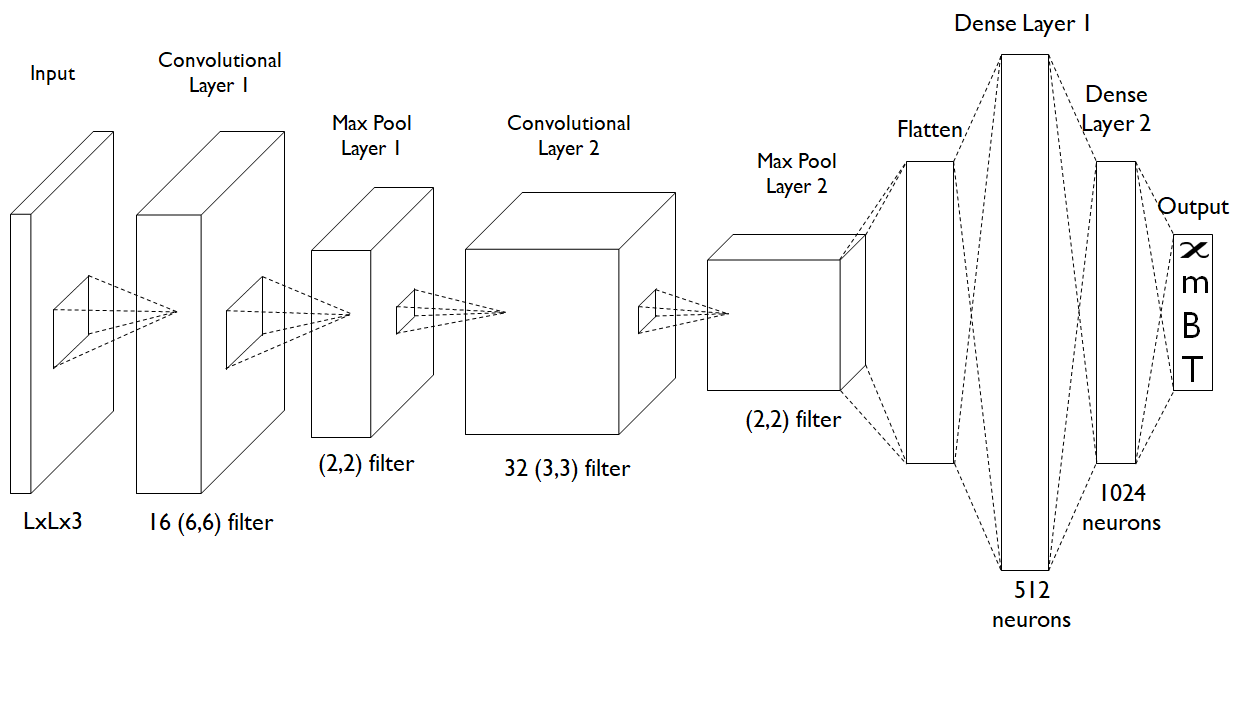
\includegraphics[scale=0.35]{fig1.png}
\caption{Schematic diagram of the ML architecture used in this work. See main text for explanation.}\label{fig:1}
\end{figure}

The use of ML as a supplement to the analysis of experimental data received very little attention in the condensed matter context  so far, although such has been the main thrust behind its vigorous application in the collider physics community. While it may be the over-production of data that interferes with the deduction of physical principles in the collider experiment, a typical condensed matter laboratory encounters problems of a different nature, that not all of the physical information one needs for thorough characterization of the material is available. The dearth of data is illustrated, for instance, with ultrathin materials that are amenable to various surface probes, but where thermodynamic measurement poses extreme challenge. It will be helpful, if possible, to have the ML program deduce ``missing information" on the basis of the data already at hand, without going through the painful process of measuring them. In this paper, we try to demonstrate the feasibility of such idea with a specific model, used in the study of two-dimensional spiral magnets and skyrmions:
%
\ba && H_{\rm HDMZ} = -J \sum_{i\in L^2} \v n_i \cdot (\v n_{i+\hat{x}} + \v n_{i+\hat{y}} ) \nn
 & & + D \sum_i ( \hat{y} \cdot \v n_i \! \times \! \v n_{i\! +\! \hat{x}} - \hat{x} \cdot \v n_i \times \v n_{i\! +\! \hat{y}} )  - \v B \cdot \sum_i \v n_i .  \label{eq:HDMZ} \ea
%
This lattice model  consisting of Heisenberg, Dzyaloshinskii - Moriya (DM) and Zeeman terms, of strengths $J$, $D$, and $B$, describes the magnetic interaction at the interface of a magnetic layer with a non-magnetic one; spins are represented as unit vector $\v n_i$ at the site $i$. Its phase diagram, by now well-established and reproduced in Fig. \ref{fig:2}, includes the skyrmion (Sk) crystal phase over some intermediate-field and low-temperature range, flanked by spiral (Sp) phase at low field and ferromagnetic (Fm) phase at high field~\cite{nagaosa-review,skyrmion-book,jiang-review,fert-review,han-book}. The spiral state has the period $\lambda$ fixed by the ratio $D/J$~\cite{han09,han-book} according to $\sqrt{2}\tan (2\pi/\lambda)  = D/J$, which also serves as the diameter of the skyrmion. The lattice spacing $a$ on the $L\times L$ square lattice is taken to unity in the model calculation, while it is a few \AA~in actual materials.  The typical spiral and skyrmion size is several tens and hundreds of lattice constants due to the small ratio $D/J \ll 1$, but it is customary in model calculations to assume $D/J$ corresponding to a few lattice constants. One justifies this on the basis that, although physical systems with their long-period structures are best described by a continuum free energy functional, in numerical studies one discretizes the continuum model and put it into the form (\ref{eq:HDMZ}) with the lattice spacing $a$ having no direct relation to the underlying physical lattice constant (see Ref. \cite{han09,han-book} for details of the discretization procedure). The lattice model parameters $J, D, B$ in (\ref{eq:HDMZ}) are renormalized from their original meaning in the continuum theory and now have the unit of energy, as does the temperature $T$ to be introduced in later Monte Carlo simulation. Conversion to physical temperature and magnetic field scales can be done with the aid of Boltzmann's constant and the Bohr magneton. Skyrmions are characterized by the topological charge, equal to the integral (or sum, if on a discrete lattice) of the spin chirality. The importance of topologically protected skyrmions as information carriers has received enormous attention recently. Readers interested in further background on skyrmions can follow recent publication of books and reviews~\cite{nagaosa-review,skyrmion-book,jiang-review,fert-review,han-book}. Surprisingly, very little attention has been given to the utility of the ML scheme toward the analysis of skyrmion experiments (Ref. \cite{russian18} focused on the phase identification problem instead). 

Figure \ref{fig:1} shows the supervised ML architecture used in this work. The input size is $(L,L,n)$ for $L\times L$ lattice.  The training data was generated by running Monte Carlo (MC) simulation on the model Hamiltonian (\ref{eq:HDMZ}) with $D/J=\sqrt{6}$, corresponding to the spiral period $\lambda=6$. This represents a convenient choice of length scale, not necessarily corresponding to actual period of the spiral in the experiment. Later we will show how the data generated at other length scales can be coarse-grained and transformed to a data set with  ``effective" lattice spacing equal to 6. We performed the ML training in three different ways using the $z$-component, $xy$-components, and full $xyz$-components of the magnetization vector $\v n_i$ generated by MC simulation. Roughly 200 training configurations are generated for each point of the $(B, T)$ grid covering the entire phase diagram shown in Fig. \ref{fig:2}: $0 \le B \le 4$ and $0.03 \le T \le 2$. For each $B$, the temperature interval was divided into 40 steps using adaptive scheduling, {\it i.e.} exponentially decaying step size with a decay rate of 0.1, giving a total of 20 steps. With 17 uniformly spaced magnetic field values, we drew 100 MC configurations at each $(B,T)$, for a total of $20 \times 100\times 17 = 34,000$ training sets. Training with much larger training set of 330,000 configurations did not change the final results. Both the fineness of the grid spacing and the number of training configurations were such that no further improvement in the performance was possible.
Testing configurations are picked from the same model, but with a separate MC run to generate them.

To ensure that the natural periodicity of the model (\ref{eq:HDMZ}) is faithfully understood by the machine, an initial convolutional neural network (CNN) layer with 16 filters, each of size 6$\times$6, was used. It was followed by the Max Pool layer of 2$\times$2 filter size, then by a second CNN layer with 32 (3$\times$3) filters.  The 3$\times$3 was chosen out of trial-and-error for the best results. Batch Normalization and Dropout Regularization accompanied both CNN layers. After applying the second Max Pooling to reduce the size, the data was fed through two Dense Neural Network (DNN) layers containing 512, 1024 neurons respectively, which then led to the output layer. Batch normalization and Dropout Regularization are applied to outputs from each DNN layer. Leaky ReLu was employed as the activation function with $\alpha=0.1$, except for the output layer where a sigmoid function was used. Adam optimizer and Learning Rate Scheduler were applied to enhance the training speed.  The training input data was arranged in terms of the local unit vector $\v n_i$, not in terms of the two angles which characterize it, due to the poorer performance in the latter case. The architecture consisting purely of the DNN layer as in Ref. \cite{russian18} generally did not work as well as the one involving also the CNN filter layers. Further minute changes in the architecture had little impact on the overall quality of final results. Exhaustive discussion of the CNN, DNN, and other nomenclature can be found in several recent books~\cite{bishop,goodfellow} and on online courses~\cite{ng}.

\begin{figure}[h]
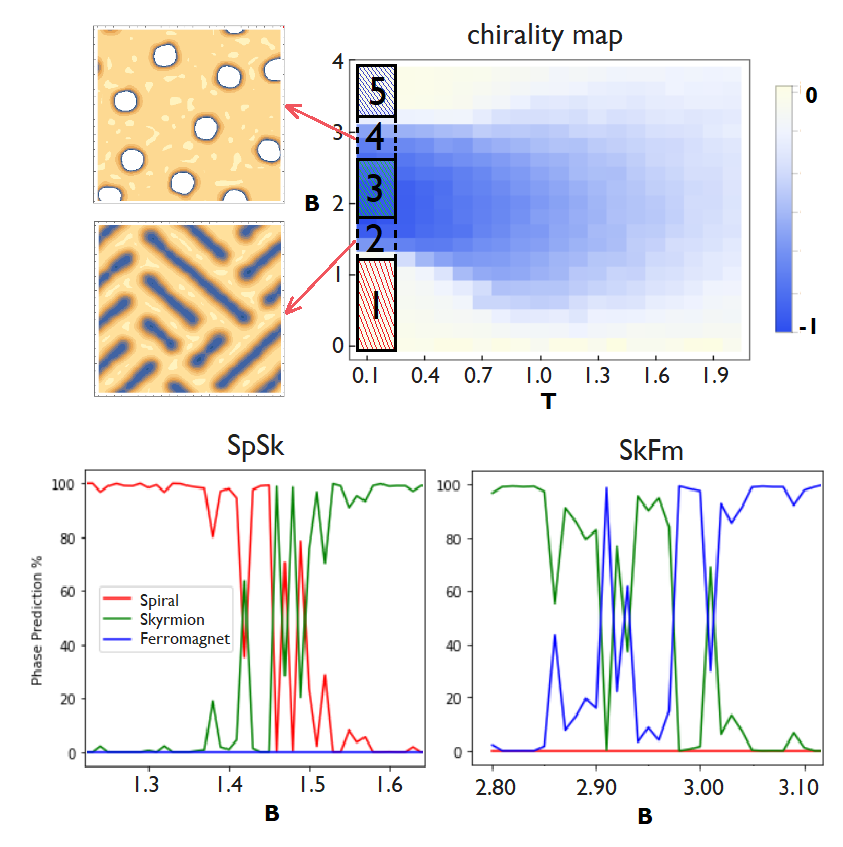
\includegraphics[scale=0.5]{fig2.png}
\caption{(top) Spin chirality $\chi$ in the $(T,B)$ plane obtained by MC calculation on the HDMZ Hamiltonian (\ref{eq:HDMZ}). Color scale represents the normalized value of the chirality. Boxes 1, 3, and 5 (2 and 4) represent regions where training (testing) data were taken for label predictions. Two configurations on the left show a typical SpSk and SkFm mixed state, respectively. The $z$-component of the local magnetization is used for the plots. (bottom) Probability of phase predictions in the SpSk and SkFm phases. The numbers represent averages over the testing set in the temperature interval $T\in[0.03,0.25]$ at the same $B$ value. The irregularities are not artifacts of the small data size.}\label{fig:2}
\end{figure}

Although the phase identification problem is not the main issue in this work as other reports already exist~\cite{russian18}, we do note an interesting aspect of the model (\ref{eq:HDMZ}) which is absent in most models studied in recent years and not amply addressed in the previous work~\cite{russian18}. Due to the substantial co-existence region both for the mixture of spiral and skyrmion (SpSk), and of skyrmion and ferromagnetic (SkFm) phases, we can categorize the overall low-temperature phase diagram in terms of five states (Sp, SpSk, Sk, SkFm, Fm), indicated as boxes numbered 1 through 5 in Fig. \ref{fig:2}. To see how the ML would fare against such a conspicuous mixed phase, we first did the ML training for MC configurations drawn from boxed regions 1, 3, 5 (three pure states). One-hot encoded labels were used to represent different phases: (1,0,0) for Sp, (0,1,0) for Sk, and (0,0,1) for Fm. Afterwards, configurations drawn from boxes 2, 4 (two mixed states) were fed to the program, demanding that it decides which of the three phases they belong to. Binary cross entropy was used as the loss function. The answers given for each test configuration by the machine were averaged over and shown as probabilities for Sp, Sk, and Fm phases  in Fig. \ref{fig:2}. Despite the fact that each data point in the figure represents an average over $2,000$ test configurations and that extremely fine steps in magnetic field $\Delta B= 0.01$ was used, the final results are far from being smooth. Removing the CNN filters did not smooth the outcome either. In contrast, a smooth variation in the probability from 1 (ordered phase) to 0 (disordered phase) was found in models with a second-order phase transition \cite{wang16,melko17,tanaka17,scalettar17,wetzel17,kim18,zhai17,scalettar17,beach18}.
The ``failure" of the ML algorithm in recognizing and characterizing mixed phases around the first-order phase transition was not appreciated in earlier investigation of the same model~\cite{russian18}. 

The two main order parameters of the phase diagram in the model (\ref{eq:HDMZ}) are the average spin chirality and the magnetization; the spin chirality becomes prominent in the skyrmion phase, the magnetization in the ferromagnetic phase, and the spiral phase supports neither. A discrete version of the spin chirality is the solid angle subtended by three adjacent spins, given by~\cite{berg81,zang16,han-book}
%
\ba \tan \left( {\chi_{ijk} \over 2} \right)  = {\v n_i \cdot \v n_j \times \v n_k \over 1 + \v n_i \cdot \v n_j + \v n_j \cdot \v n_k + \v n_k \cdot \v n_i }  . \label{eq:discrete-chi}\ea
%
In the smoothly-varying limit ($\v n_i \cdot \v n_j \approx 1$) one recovers the familiar expression $\chi_{ijk} = \v n_i \cdot \v n_j \times \v n_k /2$, which upon taking $j = i + a \hat{x}$ and $k = i + a\hat{y}$ and $a\rightarrow 0$ gives $\chi_{ijk} = a^2 \v n \cdot (\partial_x \v n \times \partial_y \v n)/2$. The spatial averages $\sum_{i} ( \chi_{i, i+\hat{x}, i+\hat{y}} + \chi_{i, i-\hat{x}, i-\hat{y}} ) /L^2 =\chi$ and $m =\sum_i n_i^z /L^2$  define the spin chirality and the magnetization, respectively. We propose to train the algorithm on the {\it features} of the data such as $\chi$ and $m$ (mechanical quantities), as well as the magnetic field $B$ and temperature $T$ (thermodynamic quantities). Here, the mean-squared error function was used as the loss function. Training configurations were drawn from the entire phase diagram in Fig. \ref{fig:1}. After training, 40,000 configurations were freshly generated to compare the machine-predicted $(\chi,m, B, T)$ against their actual values. Figure \ref{fig:3} gives the comparison of the original and machine-predicted $(\chi, m, B, T)$. Good agreements are found on all four quantities. Estimation of the error is given in the Supplementary Material (SM)~\cite{SM}. We obtained very similar quality of errors from both definitions of the spin chirality (\ref{eq:discrete-chi}) or its smooth form $\chi_{ijk} = \v n_i \cdot \v n_j \times \v n_k /2$ (Note an alternative definition of the spin chirality was adopted in Ref.~\cite{pujol15}). Results shown in the figures are based on the smooth form, which is slightly easier to compute numerically. In short, the algorithm has successfully figured out a recipe to extract $(\chi, m, B, T)$ values implicit in the spin configuration. Most remarkably, equally good predictions were possible for all three types of training data sets -  $xyz$, $xy$, and $z$ - meaning that the test image consisting of only the $z$-component of local magnetization was sufficient to predict the correct spin chirality $\chi$, which ordinarily requires the full knowledge of spin components for computation.

\begin{figure}[h]
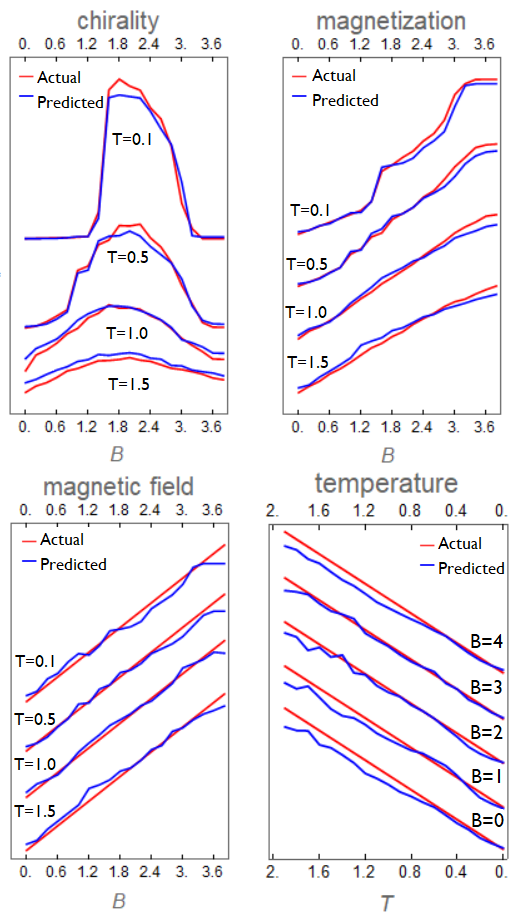
\includegraphics[scale=0.35]{fig3.png}
\caption{Machine-predicted values of $(\chi, m, B, T)$ compared to their actual values in red. Predicted values are obtained from algorithms trained on the full $xyz$, $xy$-only, and $z$-only components of the local magnetization. Different curves are offset for clarity.}\label{fig:3}
\end{figure}

The successful prediction of spin chirality based on $xy$- and $z$-only inputs, or of magnetization based on $xy$-input alone, holds interesting potential for application of ML program in the actual experiment. 
Consider two prominent imaging techniques currently under use to study skyrmion matter: Lorentz transmission electron microscopy (LTEM) \cite{tokura10} and magnetic force microscopy (MFM) \cite{pana17}. Each of them specializes in imaging the in-plane $(n^x_i , n^y_i )$ and perpendicular ($n^z_i$) components of the local magnetization. The data provided by LTEM and MFM is thus $xy$- and $z$-type, respectively.  Given the raw data, it is impossible to determine the spin chirality directly, nor to deduce the average magnetization from the LTEM data. With the ML program we developed, it appears within reach to compute both $\chi$ and $m$ with existing, partial experimental inputs. Achieving this, however, would require the establishment of a careful protocol by which the raw experimental data is converted to the machine-ready data set. 

\begin{figure}[t]
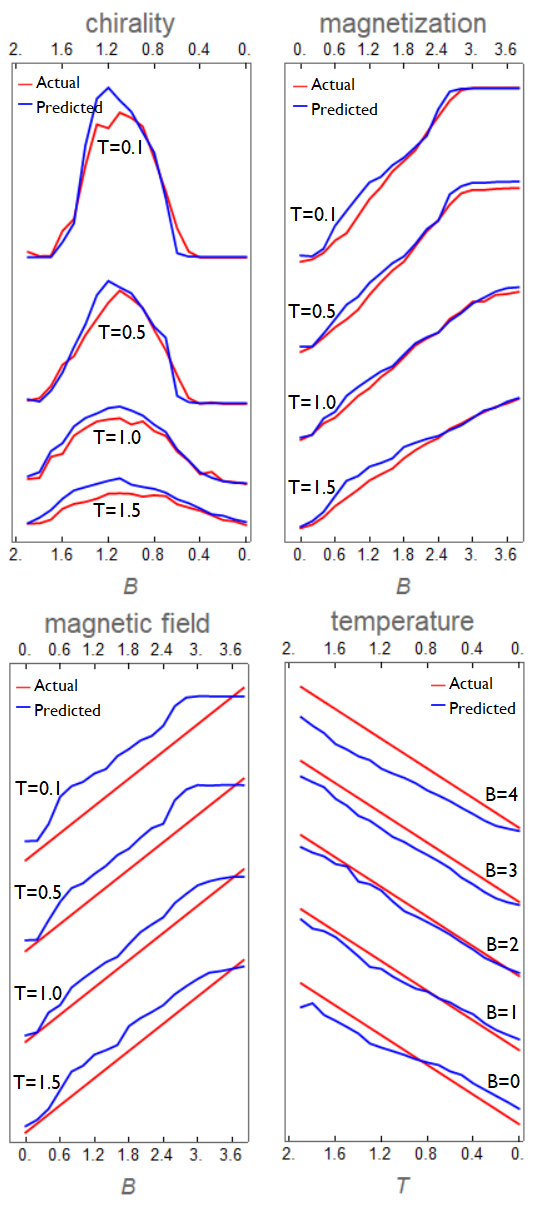
\includegraphics[scale=0.36]{fig5.png}
\caption{Top row: Machine-predicted values of $(\chi', m' )$ after coarse-graining and rescaling the original data with $b=2$. Red curve is from applying $\chi$ and $m$ formulas to pre-scaling data; blue dots are machine predictions based on renormalized input of $\v n'_i$. Middle row: Machine-predicted values $(B', T')$ vs. $(B, T)$ for $b=2$. $B'/B$ and $T'/T$ are approximately constant. Bottom row: Inference of scaling exponents from $\ln (B'/B )$ (and $\ln (T' /T)$ vs. $\ln b$ plots. Least-square fit gives slopes 2.32 and 0.73, respectively. } \label{fig:5}
\end{figure}

An obvious obstacle seems to be the vastly different length scales between experimentally-available and theoretically-generated data sets. For one, the typical size of actual skyrmion or spiral, measured in terms of physical unit-cell spacings, is 1-2 orders of magnitude greater than the period-6 structure used in our training. One way to bridge the gap in the length scales is to use coarse-graining procedure on the experimental data to match the renormalized length scale with the one used in the training. This way, the LTEM/MFM data would become compatible with the existing algorithm. Access to raw experimental data is currently not available to the authors, but one can opt for the following  proxy: in the previous ML tryouts, both the training and the test sets were generated with the same period ($D/J=\sqrt{6}$); this time, we adopt several $D/J$ values compatible with the spiral periods $\lambda=12, 18, 24$, and generate MC configurations on $L=48, 72, 96$ lattices, respectively. The MC configurations are subsequently coarse-grained according to the simple scheme, $\v n'_i = \sum'_i \v n_i / | \sum'_i \v n_i  |$, where the sum $\sum'_i$ is over the $b\times b$ block of original spins, to produce the renormalized spin configuration $\v n'_i$ on $24\times24$ lattice with the common renormalized period 6 by using $b=2,3,4$ for $\lambda=12, 18, 24$, respectively. We pose a scaling hypothesis akin to the one in real-space renormalization; one anticipates the predictions $(\chi',  m',  B' , T')$ for the renormalized spins $\{ \v n'_i \}$ to be related to $(\chi, m, B, T)$ of the original spin configuration $\v n_i$ through some scaling relation, e.g. $\chi'/\chi = b^{\#}, B'/B = b^{\#}$ with appropriate exponents $\#$. As shown in Fig. \ref{fig:5} we find $\chi' \approx \chi$ and $m' \approx m$ independent of $b$, but the ratio  $B'/B$  and $T'/T$ obey an approximate scaling relation $B'/B \approx b^{2.32}$ and $T'/T \approx b^{0.73}$. The linear fit on a log-log scale is fairly good (errors are estimated in SM~\cite{SM}), which brings us to suspect that scaling should work even at other, non-integer values of $b$. It means that even with just one period $\lambda$ used in the training, the ML program is capable of producing reliable predictions for MC configurations - and even experimental data - at other, arbitrary  $\lambda$. 

Experimental situation is still more complicated than what the simplified model (\ref{eq:HDMZ}) captures. A most obvious complication is the disorder effect, coming from inhomogeneities in the interaction parameters of the Hamiltonian or local anisotropy terms we ignored so far. The predictive capacity of ML would be much reduced if the it works well only on test  configurations generated by the exact same model from which training set was generated in the first place. Luckily, the numerical experiment presented below shows that the ML program trained on the pristine model continues to give reliable predictions for test configurations obtained from models with disorder. Replace the dirty model configurations by the actual experimental images (which always come from imperfect samples), we come to conclude that ML could give reliable predictions from messy experimental data as well.

\begin{figure}[t]
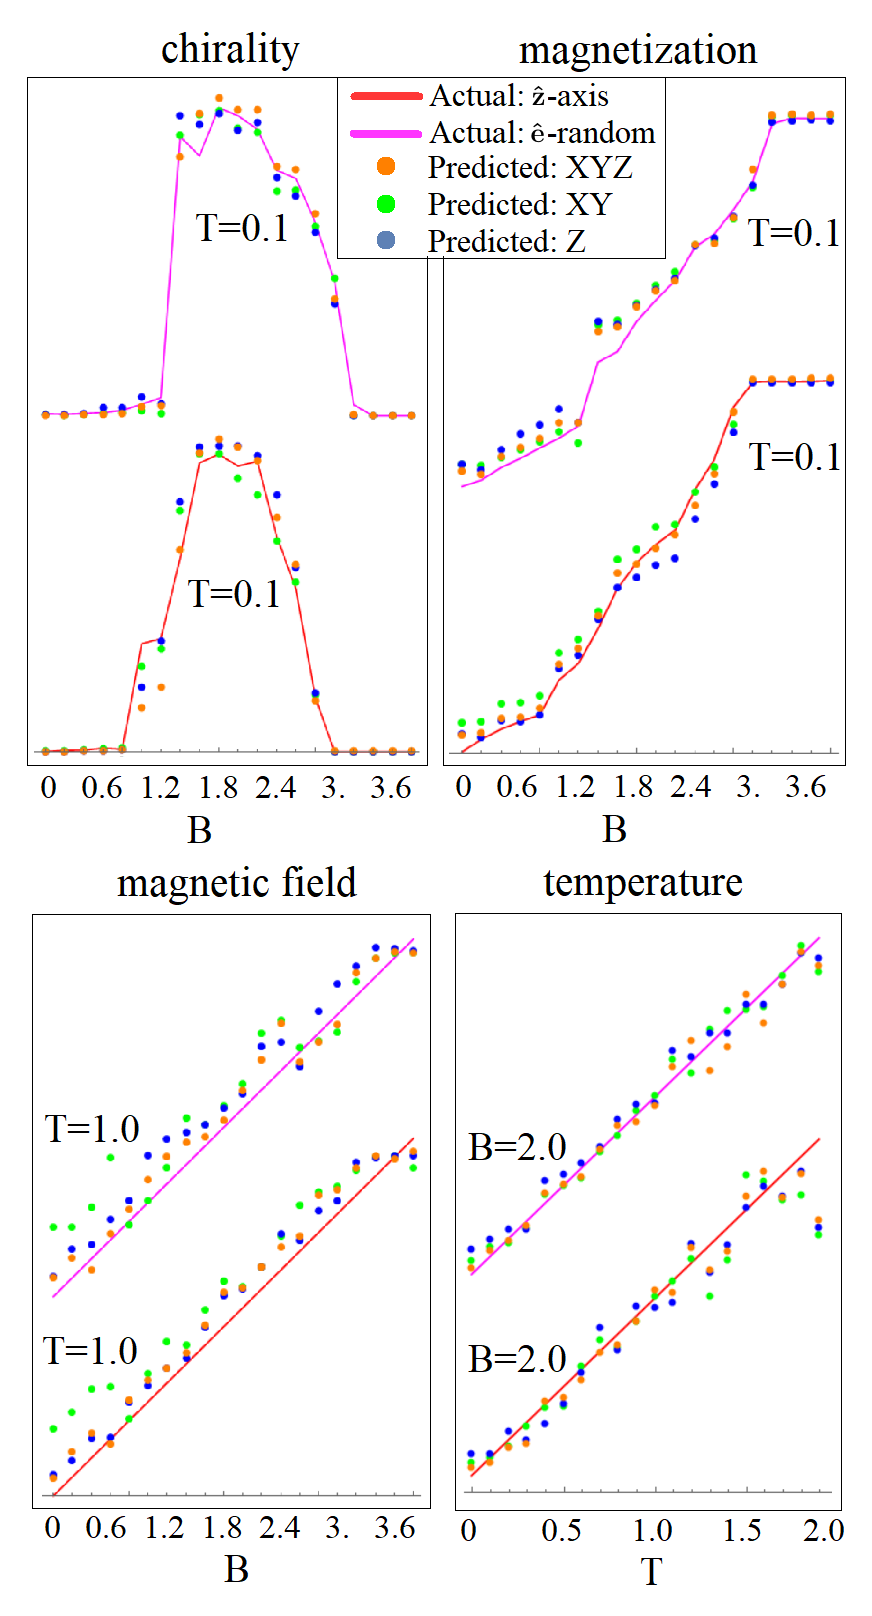
\includegraphics[scale=0.36]{fig4.png}
\caption{ML prediction of $(\chi, m, B, T)$ for MC configurations generated by $H_{\rm HDMZ}+ H_1$, and $H_{\rm HDMZ} + H_2$, with $(K,p)=(1, 0.5)$ for both models.  All three input data types ($z$, $xy$, $xyz$) give equally good predictions. Error estimation is given in SM~\cite{SM}. } \label{fig:4}
\end{figure}


We consider two kinds of disorder terms to add to the HDMZ Hamiltonian (\ref{eq:HDMZ}):
%
\ba H_{1} = -K \sum_{i \in {\rm ran}} (\hat{z} \cdot \v n_i )^2 , ~~ H_2 = - K \sum_{i \in {\rm ran}} (\hat{e}_i \cdot \v n_i )^2 .  \ea
%
In $H_1$, easy $z$-axis magnetic anisotropy of strength $K$ is added at the random sites occupying a fraction $p$ of the whole lattice. In $H_2$, the anisotropy orientation $\hat{e}_i$ is also random. A new batch of test configurations has been generated by doing MC on either  $H_{\rm HDMZ} + H_1$ or $H_{\rm HDMZ} + H_2$. We do not, however, generate a new ML algorithm trained on these new configurations. The newly-generated MC configurations are simply fed to the existing program, trained on the disorder-free model, and predictions for $(\chi, m, B, T)$ are demanded. As before, three different input types ($z$, $xy$, and $xyz$) have been used on three different ML programs. Figure \ref{fig:4} shows the outcome of such investigation. In essence, actual $(\chi, m, B, T)$ values of the test configurations with disorder are faithfully reproduced across all three data and ML types. Our numerical experiment suggests that the predictive power of ML remains universal across a range of disorder potentials. Overall errors in the predicted values of $(\chi, m, B, T)$ against the actual ones are tabulated in SM~\cite{SM}. 

We have demonstrated the versatility of the ML program in predicting physical quantities under a variety of circumstances: (i) only partial data set is available ($xy$- or $z$-component only), (ii) different length scales exist in the training and testing data sets, (iii) impurities exist. While the ultimate utility of the protocol we propose rests on its effective use in conjunction with experimental data, and that has not yet happened, we suppose that the theoretical support given in this paper can prompt such collaboration in not too distant a future. 

This work was supported by Samsung Science and Technology Foundation under Project Number SSTF-BA1701-07.

\begin{thebibliography}{99}

\bibitem{melko16} G. Torlai and R. G. Melko, Phys. Rev. B {\bf 94}, 165134 (2016).
\bibitem{wang16} L. Wang, Phys. Rev. B {\bf 94}, 195105 (2016).
\bibitem{melko17} J. Carrasquilla and R. G. Melko, Nat. Phys. {\bf 13}, 431 (2017).
\bibitem{melko17b} P. Ponte and R. G. Melko, Phys. Rev. B {\bf 96}, 205146 (2017).
\bibitem{melko17c} A. Morningstar and R. G. Melko, arXiv:1708.04622 (2017).
\bibitem{tanaka17} A. Tanaka and A. Tomiya, J. Phys. Soc. Jpn. {\bf 86}, 063001 (2017).
\bibitem{scalettar17} W. Hu, R. R. P. Singh, and R. T. Scalettar, Phys. Rev. E {\bf 95}, 062122 (2017).
\bibitem{wetzel17} S. J. Wetzel and M. Scherzer, Phys. Rev. B {\bf 96}, 184410 (2017).
\bibitem{wetzel17b} S. J. Wetzel, Phys. Rev. E {\bf 96}, 022140 (2017).
\bibitem{iso18} S. Iso, S. Shiba, and S. Yokoo, Phys. Rev. E {\bf 97}, 053304 (2018).
\bibitem{kim18} D. Kim and D.-H. Kim, Phys. Rev. E {\bf 98}, 022138 (2018).
\bibitem{zhai17} C. Wang and H. Zhai, Phys. Rev. B {\bf 96}, 144432 (2017).
\bibitem{beach18} M. J. S. Beach, A. Golubeva, and R. G. Melko, Phys. Rev. B {\bf 97}, 045207 (2018).
\bibitem{zhai18} C. Wang and H. Zhai, Front. Phys. {\bf 13}, 130507 (2018).
\bibitem{russian18} I. A. Iakovlev, O. M. Sotnikov, and V. V. Mazurenko, Phys. Rev. B {\bf 98}, 174411 (2018).
\bibitem{nagaosa-review} N. Nagaosa and Y. Tokura, Nature Nanotech. {\bf 8}, 899 (2013).
\bibitem{skyrmion-book} J. P. Liu, Z. Zhang, and G. Zhao, {\it Skyrmions: topological structures, properties, and applications} (CRC Press, 2016)
\bibitem{jiang-review} W. Jiang, G. Chen, K. Liu, J. Zang, S. G. E. Velthuis, and A. Hoffmann, {\it Phys. Rep.} {\bf 704},1 (2017).
\bibitem{fert-review} A. Fert, N. Reyren, and V. Cros, Nature Reviews Materials {\bf 2}, 17031 (2017).
\bibitem{han-book} J. H. Han, {\it Skyrmions in Condensed Matter}  (Springer, 2017).
\bibitem{han09} S. D. Yi, S. Onoda, N. Nagaosa, and J. H. Han, Phys. Rev. B {\bf 80}, 054416 (2009).
\bibitem{bishop} C. M. Bishop, {\it Pattern Recognition and Machine Learning} (Springer, 2006).
\bibitem{goodfellow} I. Goodfellow, Y. Bengio, and A. Courville, {\it Deep Learning} (The MIT Press, 2016).
\bibitem{ng} For example, Andrew Ng's online deep learning lecture can be found at https://www.coursera.org/specializations/deep-learning
\bibitem{berg81} B. Berg and M. L\"{u}scher, Nuc. Phys. B {\bf 190}, 412 (1981).
\bibitem{zang16} Gen Yin, Yufan Li, Lingyao Kong, Roger K. Lake, C. L. Chien, and Jiadong Zang, Phys. Rev. B {\bf 93}, 174403 (2016). 
\bibitem{pujol15} H. D. Rosales, D. C. Cabra, and Pierre Pujol, Phys. Rev. B {\bf 92}, 214439 (2015).
\bibitem{tokura10} X. Z. Yu, Y. Onose, N. Kanazawa, J. H. Park, J. H. Han, Y. Matsui, N. Nagaosa, and Y. Tokura, Nature (London) {\bf 465}, 901 (2010).
\bibitem{pana17} A. Soumyanarayanan, {\it et al}., {\it Nat. Mat.} {\bf 16}, 898 (2017).
\bibitem{SM} Supplementary Material
%\bibitem{zhai18b} Y. Wu, P. Zhang, H. Shen, and H. Zhai, Phys. Rev. A {\bf 98}, 010701 (2018).

\end{thebibliography}

%\bibliographystyle{apsrev}
%\bibliography{reference}

\end{document}

The model $H(K,p) = H_{\rm HDMZ} + H_K$ represents an adiabatically connected family of Hamiltonians as long as $K$ is sufficiently small compared to other energy scales. It is interesting to ask whether the ML algorithm, trained solely on  configurations drawn from $H(0,0)= H_{\rm HDMZ}$, can have predictive power over those generated from arbitrary $H(K,p)$. It is also a pragmatic question, when it comes to addressing the machine's predictive power over the experimental data, as real materials are never free of inhomogeneities and one does not have the {\it a priori} knowledge of the governing Hamiltonian. A large number of configurations at the $(K,p)$ values shown in Table \ref{tab:PBC} was generated by MC and tested by the ML algorithm, previously  trained solely on the pristine Hamiltonian $H_{\rm HDMZ}$. As shown as extensive data sets in SM, very good fits of all features $(\chi, m, B, T)$ were obtained. The error in the prediction can be quantified by measuring $\Delta X \! \equiv \!  \sum_{i=T,B} \! | X_{\rm pred.} \! - \! X_{\rm act.} | / 400 $, where 400 refers to the total number of $(T,B)$ steps used in the generation of the test set, and $X=\chi, m, B, T$. Table \ref{tab:PBC} shows the mean errors in $(\chi, m, B, T)$ for several $(K,p)$ values. Both $\Delta \chi$ and $\Delta m$ remain less than 0.05 as $K$ grows from 0 to 2 (recall $J=1$ and $D=\sqrt{6}$). Note that $\chi$ and $m$ have the maximum size of 1. On the other hand, there is a systematic growth in $\Delta B$ and $\Delta T$ as $K$ becomes larger.

\begin{table}[htb]
\begin{tabular}{ | ccc || ccc  cc  cc  cc |}
\hline
 & $(K, p)$ & & & $\Delta\chi$ &  & $\Delta m$ &  & $\Delta B$ & & $\Delta T$ & \\ \hline
 & $(0,0)$  &  & & 0.026 & & 0.027 & & 0.032 & &  0.028 & \\ \hline
 & $(1,0.5)$ & & & 0.030 & & 0.029 & & 0.060 & & 0.037 & \\ \hline
 & $(1,1)$   & & & 0.038 & & 0.024 & & 0.087 & & 0.066 & \\ \hline
 & $(2, 0.5)$ & & & 0.042 & & 0.025 & & 0.083 & & 0.064 & \\ \hline
 & $(2,1)$ & & & 0.042 & & 0.024 & & 0.152 & & 0.100 & \\ \hline
\end{tabular}\label{tab:PBC}
\caption{Averaged variance between predicted and actual values of $(\chi, m, B, T)$.}
\end{table}


We plot predicted values $B_{\rm pred.}$ against the actual $B$ in Fig. \ref{fig:4}(a) for several $(K,p)$'s. There is an approximate linear relationship in $B_{\rm pred.}$ against $B$, at least until $B_{\rm pred.}$ reaches saturation, with the slope that grows almost linearly with $K$, as shown in Fig. \ref{fig:4}(b). The effect of the added anisotropy can be qualitatively understood within the mean-field picture by replacing $K  \sum_{i \in {\rm random}}  (n^z_i )^2$ with $2K p m \sum_{i \in L^2} n^z_i$, where $p$ is the impurity fraction. Assuming the magnetization $m$ depending linearly on $B$, $m = \alpha B$, the overall effect of the random anisotropy term is to replace the external field $B$ by the effective one, $B_{\rm eff} = (1+ 2K p\alpha ) B$. The machine, having been trained solely on pristine $H_{\rm HDMZ}$, knows nothing of the impurity effect {\it a priori} and ``erroneously" predicts the renormalized $B_{\rm eff}$ for the input, thereby incidentally divulging the discrepancy between the training and testing Hamiltonian.

Such expectations are consistent with our numerical analysis of Fig. \ref{fig:4}(b), showing almost linear increase in the slope of $B_{\rm pred.}$ with $K$. To further prove this picture we obtain $\alpha$ independently from linear fits to predicted $m$ values such as shown in SM Fig. 4. The two ways of extracting the susceptibility $\alpha$ agree very well. The $\sim 2$ times difference in the estimated slopes for $p=0.5$ and $p=1$ data are consistent with the mean-field picture of $B_{\rm eff}$, as shown in Fig. \ref{fig:4}(b). The under-estimation of the temperature by the machine, as shown in SM figure 2, can be also understood, qualitatively, as a result of $K$ having the tendency to stiffen the spins and align them. At the same bare temperature $T$, configurations generated at finite $K$ tend to have more alignment of spins, which is ``erroneously" seen by the machine to be the consequence of lesser effective temperature $T_{\rm eff} < T$. Our numerical experiment demonstrates how well the neural network can respond to perturbations in the model~\cite{zhai18b}.


